% Options for packages loaded elsewhere
\PassOptionsToPackage{unicode}{hyperref}
\PassOptionsToPackage{hyphens}{url}
\PassOptionsToPackage{dvipsnames,svgnames*,x11names*}{xcolor}
%
\documentclass[
  10pt,
  dvipsnames,enabledeprecatedfontcommands]{scrartcl}
\usepackage{amsmath,amssymb}
\usepackage{lmodern}
\usepackage{ifxetex,ifluatex}
\ifnum 0\ifxetex 1\fi\ifluatex 1\fi=0 % if pdftex
  \usepackage[T1]{fontenc}
  \usepackage[utf8]{inputenc}
  \usepackage{textcomp} % provide euro and other symbols
\else % if luatex or xetex
  \usepackage{unicode-math}
  \defaultfontfeatures{Scale=MatchLowercase}
  \defaultfontfeatures[\rmfamily]{Ligatures=TeX,Scale=1}
\fi
% Use upquote if available, for straight quotes in verbatim environments
\IfFileExists{upquote.sty}{\usepackage{upquote}}{}
\IfFileExists{microtype.sty}{% use microtype if available
  \usepackage[]{microtype}
  \UseMicrotypeSet[protrusion]{basicmath} % disable protrusion for tt fonts
}{}
\usepackage{xcolor}
\IfFileExists{xurl.sty}{\usepackage{xurl}}{} % add URL line breaks if available
\IfFileExists{bookmark.sty}{\usepackage{bookmark}}{\usepackage{hyperref}}
\hypersetup{
  pdftitle={Boosting Legal Probabilism},
  pdfauthor={Marcello Di Bello and Rafal Urbaniak},
  colorlinks=true,
  linkcolor=Maroon,
  filecolor=Maroon,
  citecolor=Blue,
  urlcolor=blue,
  pdfcreator={LaTeX via pandoc}}
\urlstyle{same} % disable monospaced font for URLs
\usepackage{graphicx}
\makeatletter
\def\maxwidth{\ifdim\Gin@nat@width>\linewidth\linewidth\else\Gin@nat@width\fi}
\def\maxheight{\ifdim\Gin@nat@height>\textheight\textheight\else\Gin@nat@height\fi}
\makeatother
% Scale images if necessary, so that they will not overflow the page
% margins by default, and it is still possible to overwrite the defaults
% using explicit options in \includegraphics[width, height, ...]{}
\setkeys{Gin}{width=\maxwidth,height=\maxheight,keepaspectratio}
% Set default figure placement to htbp
\makeatletter
\def\fps@figure{htbp}
\makeatother
\setlength{\emergencystretch}{3em} % prevent overfull lines
\providecommand{\tightlist}{%
  \setlength{\itemsep}{0pt}\setlength{\parskip}{0pt}}
\setcounter{secnumdepth}{5}
%\documentclass{article}

% %packages
\usepackage{booktabs}
\usepackage[left]{showlabels}
\usepackage{multirow}
\usepackage{subcaption}

\usepackage{graphicx}
\usepackage{longtable}
\usepackage{ragged2e}
\usepackage{etex}
%\usepackage{yfonts}
\usepackage{marvosym}
\usepackage[notextcomp]{kpfonts}
\usepackage{nicefrac}
\newcommand*{\QED}{\hfill \footnotesize {\sc Q.e.d.}}
\usepackage{floatrow}

\usepackage[textsize=footnotesize]{todonotes}
\newcommand{\ali}[1]{\todo[color=gray!40]{\textbf{Alicja:} #1}}
\newcommand{\mar}[1]{\todo[color=blue!40]{#1}}
\newcommand{\raf}[1]{\todo[color=olive!40]{#1}}

%\linespread{1.5}
\newcommand{\indep}{\!\perp \!\!\! \perp\!}


\setlength{\parindent}{10pt}
\setlength{\parskip}{1pt}


%language
%\usepackage{times}
\usepackage{mathptmx}
\usepackage[scaled=0.86]{helvet}
\usepackage{t1enc}
%\usepackage[utf8x]{inputenc}
%\usepackage[polish]{babel}
%\usepackage{polski}




%AMS
\usepackage{amsfonts}
\usepackage{amssymb}
\usepackage{amsthm}
\usepackage{amsmath}
\usepackage{mathtools}

\usepackage{geometry}
 \geometry{a4paper,left=35mm,top=20mm,}


%environments
\newtheorem{fact}{Fact}



%abbreviations
\newcommand{\ra}{\rangle}
\newcommand{\la}{\langle}
\newcommand{\n}{\neg}
\newcommand{\et}{\wedge}
\newcommand{\jt}{\rightarrow}
\newcommand{\ko}[1]{\forall  #1\,}
\newcommand{\ro}{\leftrightarrow}
\newcommand{\exi}[1]{\exists\, {_{#1}}}
\newcommand{\pr}[1]{\ensuremath{\mathsf{P}(#1)}}
\newcommand{\cost}{\mathsf{cost}}
\newcommand{\benefit}{\mathsf{benefit}}
\newcommand{\ut}{\mathsf{ut}}

\newcommand{\odds}{\mathsf{Odds}}
\newcommand{\ind}{\mathsf{Ind}}
\newcommand{\nf}[2]{\nicefrac{#1\,}{#2}}
\newcommand{\R}[1]{\texttt{#1}}
\newcommand{\prr}[1]{\mbox{$\mathtt{P}_{prior}(#1)$}}
\newcommand{\prp}[1]{\mbox{$\mathtt{P}_{posterior}(#1)$}}



\newtheorem{q}{\color{blue}Question}
\newtheorem{lemma}{Lemma}
\newtheorem{theorem}{Theorem}
\newtheorem{corollary}{Corollary}[fact]


%technical intermezzo
%---------------------

\newcommand{\intermezzoa}{
	\begin{minipage}[c]{13cm}
	\begin{center}\rule{10cm}{0.4pt}



	\tiny{\sc Optional Content Starts}
	
	\vspace{-1mm}
	
	\rule{10cm}{0.4pt}\end{center}
	\end{minipage}\nopagebreak 
	}


\newcommand{\intermezzob}{\nopagebreak 
	\begin{minipage}[c]{13cm}
	\begin{center}\rule{10cm}{0.4pt}

	\tiny{\sc Optional Content Ends}
	
	\vspace{-1mm}
	
	\rule{10cm}{0.4pt}\end{center}
	\end{minipage}
	}
	
	
%--------------------






















\newtheorem*{reply*}{Reply}
\usepackage{enumitem}
\newcommand{\question}[1]{\begin{enumerate}[resume,leftmargin=0cm,labelsep=0cm,align=left]
\item #1
\end{enumerate}}

\usepackage{float}

% \setbeamertemplate{blocks}[rounded][shadow=true]
% \setbeamertemplate{itemize items}[ball]
% \AtBeginPart{}
% \AtBeginSection{}
% \AtBeginSubsection{}
% \AtBeginSubsubsection{}
% \setlength{\emergencystretch}{0em}
% \setlength{\parskip}{0pt}






\usepackage[authoryear]{natbib}

%\bibliographystyle{apalike}



\usepackage{tikz}
\usetikzlibrary{positioning,shapes,arrows}

\ifluatex
  \usepackage{selnolig}  % disable illegal ligatures
\fi

\title{Boosting Legal Probabilism}
\author{Marcello Di Bello and Rafal Urbaniak}
\date{}

\begin{document}
\maketitle

\hypertarget{the-book}{%
\section{The Book}\label{the-book}}

\hypertarget{brief-description}{%
\subsection{Brief Description}\label{brief-description}}

\footnotesize In one or two paragraphs, describe the work, including its
rationale, approach, and pedagogy. (This book is\ldots{} It does\ldots{}
Its distinguishing features are\ldots)

\normalsize

Can the evidence presented at trial be examined, weighed and assessed
using probability theory? Can legal decision-making and standards of
proof such as `preponderance of the evidence' or `proof beyond a
reasonable doubt' be defined using the language of probability? Does the
deployment of probability theory in assessing evidence and making
decisions improve the accuracy and fairness of legal decision-making?
Over the last fifty years, these questions have been debated in the
literature in philosophy, law, forensic science and artificial
intelligence. Legal probabilism is a research program that attempts to
demonstrate that the answers to these questions should be, by and large,
affirmative. Legal probabilists have made considerable progress, but
also faced robust skepticism by legal theorists and philosophers. Our
book `Boosting Legal Probabilism' examines the most important objections
to this research program and articulates a version of legal probabilism
that is able to address many, if not all, of these objections.

We begin with the simple version of the theory. It comprises two key
elements: first, Bayes' theorem for assessing the weight of the
evidence, and second, probability thresholds as decision criteria. This
simple version of legal probabilism is promising in many ways, but also
falls prey to several difficulties, including the problem of
conjunction, puzzles of naked statistical evidence, and the problem of
priors. Some legal probabilists have attempted to dismiss these
difficulties or downplay their significance. We confront them at face
value and show that they cannot be addressed within the confines of
simple legal probabilism. We then develop a more sophisticated theory,
what we call legal probabilism 1.02, which takes advantage of Bayesian
networks and other seminal ideas in the literature in forensic science
and artificial intelligence. `Boosting Legal Probabilism' articulates
the first comprehensive philosophical analysis of whether---and if so,
to what extent---legal probabilism 1.02 can overcome the limitations of
simple legal probabilism. We also show that the more sophisticated
version rivals in explanatory power two competing accounts of judicial
fact-finding: argumentation theory and relative plausibility. To add
precision to the claims made in the book, the analytic argument is
supplemented by computer simulations and \textbf{\textsf{R}} code
implementation.

`Boosting Legal Probabilism' is aimed at philosophers with an interest
in legal epistemology and epistemology more generally. Many of the
difficulties of legal probabilism resemble difficulties faced by
Bayesianism in epistemology. The book will also be of interest to legal
scholars who have championed applications of probability theory to
evidence law as well as scholars who have resisted this trend. Another
target audience includes computer scientists and psychologists
interested in studying evidential reasoning and decision-making under
uncertainty. Besides contributing to the literature about legal
probabilism, the book aims to introduce unfamiliar readers to the rich
interdisciplinary debate on the topic, often scattered throughout
journals and books in philosophy, law, computer science, forensic
science and psychology. `Boosting Legal Probabilism' can also be used by
legal practitioners and reformers who aim to strengthen the protection
for defendants against wrongful convictions, improve the accuracy of
trial decisions and promote a fairer criminal justice system. So the
book is aimed at scholars, advanced undergraduates, practitioners and
reformers. Some chapters present original research and require technical
background in probability theory. Others are introductory, suitable for
an advanced undergraduate course.

\hypertarget{outline}{%
\subsection{Outline}\label{outline}}

\noindent \textbf{Part I - Legal Probabilism and Its Foes}

\noindent The first part of the book will instill interest in legal
probabilism among unfamiliar readers and refresh seasoned readers about
the main points of contention. \textbf{Chapter 1} outlines simple legal
probabilism which comprises a familiar repertoire: Bayes' theorem,
likelihood ratios, probability thresholds, expected utility
maximization. This repertoire has proven useful in several ways,
especially in the assessment of explicitly quantitative evidence such as
DNA matches and other expert evidence. At the same time, as
\textbf{Chapter 2} shows, simple legal probabilism is liable to a host
of conceptual difficulties: the conjunction problem, the problem of
priors, and the paradoxes of naked statistical evidence. These
difficulties are well-known. Others are less familiar: the problem of
complexity, soft variables, the problem of unanticipated possibilities,
and the difficulty with corroboration.

The first two chapters provide the essential background for a deeper
examination of legal probabilism and the development of its more
sophisticated version. The remaining parts of the book cover two
distinct topics: evidence assessment (Part II and Part III, Chapters 3
through 10) and decision-making (Part IV and Part V, Chapters 11 through
17). This distinction reflects the fact that legal probabilism is both a
theory of evidence assessment (or evidence evaluation, evidence
weighing) as well as a theory of decision-making at trial. These two
topics are obviously intertwined in important ways, but are best kept
separate for analytical clarity.

\vspace{3mm}

\noindent \textbf{Part II - Evidence Assessment First Pass}

\noindent The second part of the book discusses in great detail two
formal tools that are essential for the legal probabilist: Bayes'
theorem and likelihood ratios. We focus in particular on how these tools
can help to assess, weigh and evaluate evidence at trial as well as what
their limitations are.

\textbf{Chapter 3} begins with Bayes' theorem and surveys many of its
applications, for example, as a tool to avoid reasoning fallacies such
as the prosecutor's fallacy and the base rate fallacy. At the same time,
its applications are also limited. As discussed in \textbf{Chapter 4},
court cases often require fact-finders to weigh several pieces of
evidence, sometimes conficting and susceptible to different
interpretations. The hypotheses that the fact-finders are asked to
evaluate in light of the evidence are structured stories or explanations
constituted by several sub-propositions. This level of complexity can
hardly be modeled by sucessive discrete applications of Bayes' theorem.
A more sophisticated machinery for evidence assessment is needed.

\textbf{Chapter 5} describes a formal tool distinct from Bayes' theorem
which many legal probabilists have found useful: likelihood ratios.
Bayes' theorem requires one to assess the prior probabilities of the
hypothesis of interest. The problem is that assessing prior
probabilities is notoriously difficult. Likelihood ratios, instead,
offer a way to evaluate the evidence presented at trial without the need
of assessing prior probabilities. We illustrate the applications of
likelihood ratios focusing on the debate about cold-hit DNA matches and
the impact of false positive probability. The chapter also examines the
weaknesses of this approach. The choice of the competing hypotheses
compared in the likelihood ratio is often a source of confusion,
manipulation and subjective judgment. Another problem is that, like
simple applications of Bayes' theorem, likelihood ratios are still
unable to model complex bodies of evidence. A further problem, as
critics have alleged, is that likelihood ratios face difficulties in
modeling the notion of evidential relevance in certain cases.

\vspace{3mm}

\noindent \textbf{Part III - Evidence Assessment More and Better}

\noindent Chapters 3 and 4 show that we need to move past simple legal
probabilism. Chapter 5 shows that likelihood ratios, while useful in
many ways, are still an unsatisfactory approach overall. The journey
toward legal probabilism 1.02 is accomplished in Part III, Chapters 6
through 10. Our analysis is informed by the following working
hypothesis. An accusation of liability must be substantiated by
providing a well-specified account---a story or narrative---of the
alleged illegal act committed by the defendant. This account consists of
several moving parts, each supported by different items of evidence. The
defense may respond by attacking the supporting evidence, the internal
consistency of the account, or by offering an alternative account. It is
this complex dynamics that we aim to formalize in the following
chapters.

We focus on two aspects of the evaluation of trial evidence which simple
legal probabilism is unable to model: first, judges and jurors often
think holistically about the evidence, say in terms of coherent stories
or explanations, without assessing the evidence by discrete applications
of Bayes' theorem or likelihood ratios; second, different pieces of
evidence interact in complex relationships, such as undercutting,
rebutting, converging, or corroborating evidence. We show that Bayesian
networks constitute the formal machinery necessary for developing a more
sophisticated legal probabilism that is able to capture these phenomena.
The key idea is that the coherence of a story as well as conflicts
between pieces of evidence can be modeled formally by corresponding
properties of, operations on, and relations between Bayesian networks.

\textbf{Chapter 6} offers a crash course on Bayesian networks with a
focus on the assessment of legal evidence. A Bayesian network comprises
a directed acyclic graph (called a DAG) that represents relations of
dependence between variables, along with conditional probability tables
corresponding to these relations. In the last decade, the literature in
artificial intelligence and forensic science has made significant
progress in modeling holistic notions such as the coherence of a story
and argument-based notions such as conflicts between pieces of evidence.
Chapter 6 surveys this literature focusing on the work of Charlotte Vlek
and Norman Fenton. Vlek, together with Bart Verheij and Henry Prakken,
proposed to model the coherence of a story by adding a node in the
Bayesian network, call it a `story node.' The story node has other nodes
as its children corresponding to the events that make up the story. In
turn, these events are linked to their supporting evidence. An example
of a Bayesian network with a story node (or scenario node to use Vlek's
terminology) is depicted below:

\begin{center}
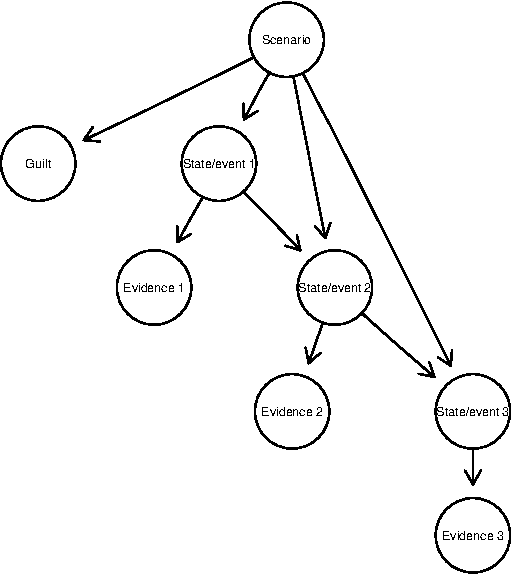
\includegraphics[width=8cm]{vlek-scenario-node.pdf}
 \end{center}

Since the story node unifies the different parts of a story, changes in
the probabilities of these parts can be used to model the notion of
coherence. The stronger the (positive) probabilistic dependence between
the different parts, the more coherent the story. To model conflicts of
evidence, a Bayesian network can be built that comprises two competing
stories, say, one story put forward by the prosecution and another by
the defense, each supported by their own evidence. The network would
specify that these stories are incompatible and cannot be true
concurrently. Another approach to model conflicting evidence and
competing stories was developed by Norman Fenton and his research group.
Separate stories are represented by separate Bayesian networks, and
Bayesian model comparison is then used for assessing the comparative
evidential support of the competing stories.

\textbf{Chapter 7} focuses on Vlek's story node approach as an account
of coherence. The chapter contains a critical argument followed by a
positive proposal. We show that adding a story node by fiat---without
any good reason for supposing that the different parts of the story are
connected other than being part of one story---introduces unnecessary
probabilistic dependencies between the elements of a story. In addition,
the story node approach is overly simplistic as an account of coherence
and fails to engage with the rich philosophical literature on the topic.
After the critical argument, the chapter articulates a more adequate
probabilistic account of coherence.
\todo{This sentence is too vague in its positive part:} Instead of
adding a story node, we show that it is more appropriate to assess the
dependence between the different parts of a story on a case-by-case
basis and build the Bayesian network accordingly. We then define a
formal notion of `story coherence' that reflects properties of the
Bayesian network used to model the evidence. We show that our formal
notion of coherence addresses the objections against probabilistic
accounts of coherence in the philosophical literature.
\raf{M: ANYTHING ELSE TO DESCRIBE THE POSITIVE ACCOUNT?}

\textbf{Chapter 8} focuses on conflicts between pieces of evidence.
Neither Vlek's story node approch nor Fenton's model comparison approach
adequately capture how pieces of evidence and competing stories may
conflict with one another. It is too simplistic to posit that the
complex adversarial dialectic that takes place in a trial could be
modeled by averaging different Bayesian networks (Fenton) or postulating
relationships of incompatibility between different story nodes (Vlek).
We need an account of more fine-grained notions, such as undercutting
and rebutting evidence, and more generally we need an account of how
cross-examimation operates at trial. What cross-examination often
accomplishes is not so much the creation of an alternative story, but
rather, the reinterpretation of an existing story by supplying
additional information. We show that this process of reintepretation can
be represented formally as the refinement of an existing Bayesian
network. Conflicts between pieces of evidence such as undercutting and
rebutting can be modeled by drawing additional arrows between evidence
nodes and hypothesis nodes.

The reverse of the phenomenon of conflicting evidence is that of
converging evidence, in particular, the fact that one piece of evidence
corroborates another. Corroboration has been the focus of extensive
scholarly debate often independently of the debates within legal
probabilism. \textbf{Chapter 9} surveys the literature on corroboration
and the main difficulties that have been leveled against proposed
probabilistic accounts. The chapter then formalizes a notion of
corroboration using Bayesian networks that overcomes most of the
difficulties of exisisting accounts.
\raf{M: ANYTHING ELSE TO DESCRIBE THE POSITIVE ACCOUNT?}

\textbf{Chapter 10} draws some general morals after comparing legal
probabilism 1.02---as fomulated in the previous two chapters---to other
accounts of judicial fact-finding, in particular, argumentation theory
and relative plausibility. Argumentation theory is well suited to model
conflicts between evidence, but cannot easily model the fact that
evidence may conflict more or less strongly with other evidence. Unlike
argumentation theory, legal probabilism 1.02 offers an account of
evidential support, conflict and convergence that captures how these
relations come in degrees of strength. The other competing theory we
consider, relative plausibility, is often criticized because the defense
lawyer need not present a full-fledged alternative story. Without
settling this controversy, we note that legal probabilism 1.02 is
flexible enough to model competing stories (in agreement with relative
plausibility) or model conflicts without the need to construct a
full-fledged alternative story (as critics of relative plausibility
prefer).

Legal probabilism 1.02 can still be challenged because of its
questionable emprical adequacy since judges and jurors hardly follow
probability theory. Nevertheless, we emphasize how legal probabilism
1.02 offers a richer account of evidential support beyond what critics
have recognized. Susan Haack, for example, criticized legal probabilism
for its monodimensional account of evidential support. This is true of
simple legal probabilism in which evidential support is modeled by the
posterior probability of a hypothesis given the evidence or the
likelihood ratio. Legal probabilism 1.02, however, offers a richer
account. In it, evidential support also depends on the degree of
specificity and coherence of the story put forward, and the extent to
which the supporting evidence withstands objections. These
features---specificity and coherence, as well as resistance to
objections---can serve to formulate decision criteria that are not
unidimensional thresholds. Criteria for trial decisions are discussed
more extensively in the next part of the book.

\vspace{3mm}

\noindent \textbf{Part IV - Decision-making}

\noindent The third part of the book examines trial decision-making,
specifically, to what extent standards of proof such as `preponderance
of the evidence' and `proof beyond a reasonable doubt' can be understood
through the lenses of probability theory. There has been a spur of
research arguing that legal probabilism is unfit to model standards of
proof. But this research often holds a narrow view of legal probabilism.
We show that the version formulated in the previous chapters of the book
provides an adequate framework for theorizing about standards of proof.

\textbf{Chapter 11} examines different strategies for theorizing about
standards of proof using probabilistic language. We begin with the most
natural decision criterion, a probability threhsold whose stringency is
determined by expected utility maximization. This account falls prey to
well-known objections, most notably, the puzzles of naked statistical
evidence and the difficulty with conjunction (discussed in greater
detail in later chapters). We then turn to alternative accounts, in
particular, the comparative strategy (Cheng) and the likelihood ratio
strategy (Dawid, Kaplow, Sullivan). Finally, we present our own
proposal. That is, the standard of proof is a function of several
criteria: the probability of liability, the specificity and coherence of
the accusatory story, the comprehensiveness of the supporting evidence
and its ability to withstand objections. We emphasize that these
criteria---probability, specificity, etc.---can be modeled using
Bayesian networks. So our proposal lies within the confines of legal
probabilism, though not the narrow version its critics have in mind. In
the following chapters, we illustrate the theoretical payoffs that come
from endorsing our proposal.

\textbf{Chapter 12} tackles the puzzles of naked statistical evidence.
This is a topic of enormous scholarly attention in the recent
philosophical literature. Our solution rests on two premises. First, an
accusation of liability should be substantiated by a well-specified
account---or story, narrative---whose moving parts are each supported by
adequate evidence. In cases of naked statistical evidence, the
probability of liability is high, but the specificity of the
accompanying narrative is suspiciously low. The second premise is that
the supporting evidence should typically be `causally grounded.' This
grounding contributes to a well-specified story and is achieved during
cross-examination by eliciting additional information about the relation
between the evidence and the alleged facts---for example, information
about the visibility conditions; the academic credential of an expert
witness; the chain of custody of a document. Interestingly, naked
statistical evidence blocks cross-examination because no undercutting
evidence can in principle be brought against it.

\textbf{Chapter 13} tackles another central problem for legal
probabilism, the difficulty with conjunction. We first provide a
detailed argument for why previous attempts in the literature on legal
probabilism have failed, focusing on the likelihood ratio approach by
Dawid and the comparative strategy by Cheng. Our proposal follows the
holistic approach by Allen and Pardo. As noted already, our working
hypothesis is that the prosecution (or the plainitiff in a civil trial)
should aim to establish a well-specified accusatory narrative whose
moving parts are supported by adequate evidence. We show how legal
probabilism can address the difficulty with conjunction so long as it
can account for holistic notions such as coherence and specificity. Once
the prosecution has accomplished that---and its case withstands
criticism---each element of the accusation is established to the
required standard if and only if the conjunction of these elements (that
is, the story as a whole) is established to the required standard.

\textbf{Chapter 14} compares our probabilistic account of
decision-making and standards of proof to other accounts in the
literature. We advance two main points of criticism. First, other
accounts are not necessarily incompatible with legal probabilism 1.02
which may in fact provide a more rigorous way to express their insights.
This point applies to foundeherentism (Hack), normic support (Smith),
argumentation theory (Sartor and Prakken) and to some extent relative
plausibility (Allen and Pardo). The second criticism we make is that
other accounts are engaged with what we might call `epistemology
fetishism'---that is, they borrow ideas in contemporary analytic
epistemology and force them onto legal-decision making. This criticism
applies in particular to knowledge accounts of legal proof. To be sure,
we might ourselves be accused of `probability fetishism'---that is,
unquestionably taking probability theory as a paradigm of rationality
and force it onto legal-decision making. Admittedly, there is no
empirical evidence that a probabilistic turn in legal decision-making
would improve trial decisions, if only because what it would mean to
`improve' trial decisions is unclear. A set of criteria are needed for
assessing the desired improvements. We tackle this normative question in
the final part of the book and show how probability theory can be of
service here.

\vspace{3mm}

\noindent \textbf{Part V - Accuracy and Fairness}

\noindent What values and objectives should trial decisions seek to
realize? What criteria and principles should guide trial decisions so
that they can further these values and objectives? The fourth part of
the book addresses these questions by focusing on improving the accuracy
and fairness of trial decisions.

As a preliminary step, \textbf{Chapter 15} surveys different values and
objectives that may inform the design of the trial system. In response
to criminal and civil wrongs, we assume that the state has, in
principle, the authority to impose punishments and decide about monetary
compensations. Given this assumption, we survey the most common values
and objectives that trial decisions should conform with: trial decisions
should be accurate; they should be fair; they should be accompanied by a
justification that is public and subject to scrutiny; they should be
reversible under appeal; they should contribute to further social
cohesion, compliance and deterrence; they should be humane and
respectful of people's dignity. We also explore to what extent these
values and objectives may be in tension with one another and to what
extent they can be subject to restrictions. The subsequent chapters
focus on two values and objectives: accuracy and fairness. We focus on
them, not because the others are not important, but because we believe
they are foundational for the others.

\textbf{Chapter 16} examines what it means for trial decisions to be
accurate and how accuracy can be promoted. There are different ways to
understand accuracy in trial decisions. We first distinguish accuracy in
the single instance and accuracy in the long run. Accuracy in the single
instance consists in the conviction of a defendant that is factually
guilty and the acquittal of a defendant that is factually innocent. A
similar definition applies to civil liability. Some have criticized the
notion of `factual guilt' on the ground that guilt is a judgment based
on evidence, not a state of affairs the exists objectively. We argue
that this view deprives trial decisions of objectivity and legitimacy.
We then turn to accuracy in the long run. In this sense, accuracy can be
understood as predictive or diagnostic. The former is the probability
that, if the defendant is found (not) liable at trial, the defendant is
actually (not) liable; the latter is the probability that if the
defendant is (not) liable, the defendant would (not) be found liable at
trial. The two notions are related but are not equivalent.
Distinguishing them has implications for how we should understand
standards of proof. To this end, we ask whether the standard of proof as
we defined in earlier chapters---consisting of multiple criteria such as
high probability of liability, narrative specificity and resistance to
objections----does in fact promote accuracy in the long run. We devise a
computer simulation that compares two models of the standard of proof.
On the first model, the standard of proof simply requires that the
defendant's liability be established with a high probability. On the
second model, the standard of proof requires, in addition to high
probability, that the narrative presented by the prosecution or the
plaintiff be reasonably specific. We compare the performance of the two
models against long run predictive and diagnostic accuracy. The first
model prevails in terms of predictive accuracy, while the second
prevails in terms of diagnostic accuracy. We argue that diagnostic
accuracy, rather than predictive accuracy, is the most adequate notion
of accuracy for assessing trial decisions. We conclude that
understanding the standard of proof as the combination of a `high
probability' and `narrative specificity' (as we have argued in earlier
chapters) is a more rational model of the standard of proof.

\raf{M: Anythign to add or remove?}

\textbf{Chapter 17} turns to the fairness of trial decisions. What does
it means for trial decisions to be fair? In a formalistic sense,
fairness merely requires that every rule be applied to all defendants in
the same way. In the substantive sense, fairness requires, in an
absolute sense, that trial defendants not be subject to excessive
burdens, and in a comparative sense, that burdens (and benefits) be
roughly equally distributed across different defendants. Substantive
fairness, in the comparative sense, can be understood as the requirement
that all defendants be exposed to roughly the same risk of mistaken
conviction (or more precisely, that the conditional probability that a
defendant, if innocent, is convicted be the same across all defendants).
Equipped with this notion of substantive comparative fairness, we
examine whether admitting certain types of evidence makes trial
decisions unfair, and to what extent trial decisions are inevitably
unfair because of structural inequalities in society. We argue that
admitting certain forms of evidence, specifically profile evidence and
group-based generalizations, tends to burden certain groups of
defendants more heavily than others, thus deteriorating the fairness of
trial decisions. We also compare, via a computer simulation, different
models of the standard of proof and examine which model is conducive to
fairer trial decisions. We show that a standard of proof that
incorporates multiple criteria---such as high probability of liability;
specificity of the narrative; resistance to objections;
comprehensiveness of the evidence---allocates burdens and benefits more
fairly across defendants than a standard of proof that simply requires
that the probability of liability be above a fixed threshold. Thus, the
multidimensional account of the standard of proof we have proposed fares
relatively well in light of normative criteria such as accuracy
(previous chapter) and fairness (this chapter).
\raf{M: Anythign to add or remove?}

\textbf{Chapter 18} draws some conclusions and points to open problems
for legal probabilism. We emphasize that our aim in the book is to show
that legal probabilism is a richer and more flexible theory that it
might seem at first. It is a theory that is able to incorporate insights
from other, possibly rival theories. Legal probabilism 1.02 can
satisfactorily address long-standing conceptual difficulties could be
satisfactorily addressed: the problem of naked statistical evidence, the
difficulty with conjunction, corroboration and cross-examination. Other
conceptual difficulties remain outstanding, such as the problem of
priors and the problem of unanticipated possibilities. Besides
furthering the academic debate, `Boosting Legal Probabilism' can be used
by legal practitioners and reformers who aim to strengthen the
protection for defendants against wrongful convictions, improve the
accuracy of trial decisions and promote a fairer criminal justice
system. We sketch how our theoretical findings can be implemented in the
trial setting, but leave a more precise articulation of the challenges
of implementation for future work.

\raf{M: ANYTHING TO ADD HERE?}

\todo{Question: don't we plan to have a chapter on the priors?}

\vspace{3mm}

\noindent \textbf{Table of contents}

\renewcommand{\labelenumi}{\Roman{enumi}}
\renewcommand{\labelenumii}{\arabic{enumii}}
\renewcommand{\labelenumiii}{\arabic{enumii}.\arabic{enumiii}}

\begin{enumerate}
\item Legal probabilism 1.01 and its foes
\begin{enumerate}

  \item The emergence of legal probabilism
  \begin{enumerate}
  \item  Famous cases
  \item  Probabilistic evidence
  \item  Trial by mathematics
  \item  Some history
  \end{enumerate}
  

  
  \item  A skeptical perspective
  \begin{enumerate}
  \item  The difficulty about conjunction
  \item  The problem of priors
  \item  Naked statistical evidence
  \item  The complexity problem
  \item  Soft variables
  \item  Corroboration
  \item  The reference class problem
  \item  Unanticipated possibilities
  \item  Non-probabilistic theories
  \end{enumerate}


\end{enumerate}
\item  Evidence assessment (first pass)


\begin{enumerate}


\setcounter{enumii}{2}
  \item  Bayes' theorem and the usual fallacies
  \begin{enumerate}
  \item  Assuming independence
  \item  The prosecutor's fallacy
  \item  Base rate fallacy
  \item  Defense attorney's fallacy
  \item  Uniqueness fallacy
  \item  Case studies
  \end{enumerate}

  
  
  \item  Complications and caveats
  \begin{enumerate}
  \item  Complex hypotheses and complex bodies of evidence
  \item Source, activity and offense level hypotheses
  \item  Where do the numbers come from?
  \item  Modeling corroboration
  \item  Stories, explanations and coherence
  \end{enumerate}

  
  \item  Likelihood ratios and relevance
  \begin{enumerate}
  \item Likelihood ratio as a measure of evidence strength
  \item The risk of false positive and its impact
  \item Hypothesis choice
  \item Levels of hypotheses and the two-stain problem
  \item Relevance and the small-town murder scenario
  \item The cold-hit confusion
  \item  Likelihood ratio and  cold-hit DNA matches
  \end{enumerate}


\end{enumerate}
\item  Evidence assessment (more and better)
\begin{enumerate}

\setcounter{enumii}{5}
\item  Bayesian Networks

  \begin{enumerate}
  \item  Bayesian networks to the rescue
  \item  Legal evidence idioms
  \item Scenario idioms
  \item Modeling relevance
  \item  Case study: Sally Clark
  \item DNA evidence
  \end{enumerate}
  
   \item Coherence
  \begin{enumerate}
  \item  Existing probabilistic coherence measures
  \item  An array of counterexamples
  \item Coherence of structured narrations with Bayesian networks
  \item  Application to legal cases
  \end{enumerate}
  
  
  \item Conflicts
  \begin{enumerate}
  \item Argumentation theory
  \item Undercutting and rebutting evidence
  \item Cross-examination
  \item Conflicting evidence in Bayesian networks
  \end{enumerate}
 
 
  \item Corroboration
  \begin{enumerate}
  \item Boole's formula and Cohen's challenge
  \item  Modeling substantial rise in case of agreement
  \item Ekel\"of's corroboration measure and evidentiary mechanisms
  \item General approach with multiple false stories and multiple witnesses
  \end{enumerate}


  \item  Towards legal probabilism 1.02
    \begin{enumerate}
    \item Outperforming competing accounts
    \item Empirical adequacy
    \item Specificity and coherence
    \item Resistance against objections 
    \item Comprehensive evidence
    \item Bayesian network implementation
    \end{enumerate}


\end{enumerate}
\item  Standards of proof
\begin{enumerate}


\setcounter{enumii}{10}
 \item  Are standards of proof thresholds?
  \begin{enumerate}
  \item  Legal background
  \item  Probabilistic thresholds
  \item  Theoretical challenges
  \item  The comparative strategy
  \item  The likelihood strategy
  \item  Probabilistic thresholds revised
  \item  Bayesian networks and probabilistic standard of proof
  \end{enumerate}


\item  Naked statistical evidence
  \begin{enumerate}
  \item  Forty years of hypothetical
  \item  Specific narratives
  \item  Cross-examination and causal grounding
  \item  Specificity, causality and Bayesian networks 
  \item  Are cold-hit DNA matches naked statistics?
  \end{enumerate}
  
  
\item  The Difficulty with Conjunction
  \begin{enumerate}
  \item  The problem
  \item  The likelihood strategy
  \item  The comparative stratgey
  \item  The holistic strategy
  \item  Complex bodies of evidence and structured narratives
  \end{enumerate}  

 \item  Other accounts 
  \begin{enumerate}
  \item  Baconian probability
  \item  Sensitivity
  \item  Normic Support
  \item  Foundherentism
  \item  Relevant alternatives
  \item  Knowledge
  \item  Relative Plausibility
  \item  Arguments
  \end{enumerate}

\end{enumerate}
\item  Accuracy and Fairness
\begin{enumerate}

\setcounter{enumii}{14}
  \item  The objectives of trial desicions
  \begin{enumerate}
  \item  Conceptual desiderata
  \item  Accurate and fair decisions
  \item  Protecting defendants
  \item  Public justification 
  \item  Revision and appeal
  \item  Dispute resolution and public deference
  \end{enumerate}




  \item  Accuracy and the risk of error
  \begin{enumerate}
  \item  Single case accuracy
  \item  Minimizing expected errors
  \item  Expected v.\ actual errors
  \item  Predictive and diagnostic accuracy
  \item  Error reduction and error distribution
  \item  Accuracy, high probability and specificity 
  \end{enumerate}


  \item  Fairness in trial decisions
  \begin{enumerate}
  \item  Procedural v.\ substantive fairness
  \item  Absolute v. comparative fairness 
  \item  Measures of fairness and measures of accuracy 
  \item  Profile evidence and group-generalizations
  \item  Structural inequalities 
  \item  A fairer standard of proof
  \end{enumerate}


\item Conclusions
\begin{enumerate}
\item  Assessing the progress made
\item  Open questions problems 
\item  To reformers and practitioners
\end{enumerate}
\end{enumerate}
\end{enumerate}

\hypertarget{outstanding-features-of-the-book}{%
\subsection{Outstanding Features of the
Book}\label{outstanding-features-of-the-book}}

\begin{itemize}
\item
  `Booosting Legal Probabilism' is divided into different parts, each
  tackling a distinct domain and level of analysis. The first half (PART
  II and PART III) examines the correct probabilistic assessment of the
  evidence. The second half examines decisions at trial. The discussion
  of decision offers a probability-based explication of the standards of
  proof that is theoretically plausible (PART IV). In addition, we also
  provide a normative justification of the proposed theory based on its
  performance in light of accuracy and fairness (PART V).
\item
  The book is interdisciplinary. It closely engages with the literature
  in philosophy (see, for example, the discussion about coherence and
  corroboration) as well as literature outside philosophy in artificial
  intelligence and forensic science (see, for example, the discussion pf
  Vlek's story node approach and Fenton's everaging).
\item
  `Booosting Legal Probabilism' is the first comprehensive sustained
  philosophical examination of legal probabilism and how it fares
  against well-known objections.
\item
  The analytical, theoretical argument in defense of legal probabilism
  is accompanied by an \textbf{\textsf{R}} code implementation. This
  underscores the theoretical, practical and computational aspiration of
  `Boosting Legal Probabilism.'
\item
  The book is suitable for different audiences with different interests.
  It is partly introductory and partly describing original research by
  the authors. Instead of reading the entire book, one could follow
  different tracks. One could read the book to learn about the proof
  paradoxes (Chapter 2, 11, 12 and 13), Bayesian networks for evidence
  assessment and decision-making (Chapters 6 through 11, legal
  probabilism and its difficulties (Chapter 1, 2, 3, 4 and 11), the
  accuracy and fairness of trial decisions (Chapters 14, 16 and 17),
  etc. We will make sure to describe several tracks that readers could
  follow depending on their interests.
\end{itemize}

\raf{M: What else?}

\hypertarget{apparatus}{%
\subsection{Apparatus}\label{apparatus}}

\footnotesize a. Will the book include photographs, line drawings,
cases, questions, problems, glossaries, bibliography, references,
appendices, etc.?

\footnotesize b. If the book is a text, do you plan to provide
supplementary material to accompany it? (Teacher's manual, study guide,
solutions, answers, workbook, anthology, or other material.)

\vspace{2mm}

\normalsize

Besides the customary list of references at the end, the book will
contain several graphs and plots, Bayesian networks, and other data
visualizations generated via the \textbf{\textsf{R}} package
\texttt{ggplot2} as is standard in publications in statistics and
machine learning.

Since computer simulations play an integral part in the argument, the
book will be accompanied by supplementary materials available on-line.
These materials will contain the \textbf{\textsf{R}} source code for the
simulations along with tutorials for students or readers interested in
learning the technical details.

\hypertarget{competition}{%
\subsection{Competition}\label{competition}}

\footnotesize a. Consider the existing books in this field and discuss
specifically their strengths and weaknesses. Spell out how your book
will be similar to, as well as different from, competing works.

\begin{enumerate}
\def\labelenumi{\alph{enumi}.}
\setcounter{enumi}{1}
\item
  Consider what aspects of topical coverage are similar to or different
  from the competition. What topics have been left out of competing
  books and what topics have been left out of yours?
\item
  Please discuss each competing book in a separate paragraph. (If
  possible, please provide us with the publisher and date of publication
  as well.) This information will provide the reviewers and the
  publisher a frame of reference for evaluating your material. Remember,
  you are writing for reviewers and not for publication, so be as frank
  as possible regarding your competition. Give credit where credit is
  due, and show how you can do it better.
\end{enumerate}

\normalsize

Several books in print cover topics at the intersection of evidence, law
and probability. They, however, do not have the same aims as our book.

Consider first books written by legal theories and philosophers, such as
Stein (2005), \textit{Foundations of Evidence Law}, Oxford University
Press; Ho (2008),
\textit{A Philosophy of Evidence Law: Justice in the Search for Truth},
Oxford University Press; Haack (2014),
\textit{Evidence Matters: Science, Proof, and Truth in the Law},
Cambridge University Press; Nance (2016),
\textit{The Burdens of Proof: Discriminatory Power, Weight of Evidence, and Tenacity of Belief},
Cambridge University Press; Dahlman, Stein, and Tuzet (eds.) (2021),
\textit{Philosophical Foundations of Evidence Law}, Oxford University
Press. These books offer original theories of evidence law, the
standards of proof and legal decision-making under uncertainty. They
address, from a philosophical perspective, many of the conceptual
difficulties that we examine in our book. But they do not develop a
probabilistic theory of evidence and decision-making that crucially
relies on Bayesian networks.

Many books by forensic scientists and computer scientists have
championed applications of Bayesian networks to legal evidence
evaluation, for example, Taroni, Aitken, Garbolino and Biedermann (2006)
\textit{Bayesian Networks and Probabilistic Inference in Forensic Science},
Wiley; Taroni, Bozza, Biedermann, Garbolino and Aitken (2010),
\textit{Data Analysis in Forensic Science: A Bayesian Decision Perspective},
Wiley; Fenton and Neil (2012/2018)
\textit{Risk Assessment and Decision Analysis with Bayesian Networks},
Chapman and Hall/CRC Press. These books are groundbreaking in that they
offer a detailed examination of how expert evidence can be assessed
using Bayesian networks. They, however, do not address philosophical
problems such as the problem of naked statistical evidence or the
difficulty of conjunction, nor do they aim to offer a novel theory of
the standard of proof. Unlike our book, they do not address normative
questions such as the accuracy or fairness of trial decisions.

Several books exists about Bayesian networks that are more general in
content, such as Scutari and Denis (2014),
\textit{Bayesian Networks With Examples in R}, Chapman and Hall/CRC
Press. Many books also examine how our minds rely on evidence to
understand the world and solve problems, such as Lagnado (2021),
\textit{Explaining the Evidence: How the Mond Investigates the World},
Cambridge University Press. We do not review these books in any detail.
They differ from our book mostly because they lack a focus on legal
applications.

There are books that focus exclusively on the evaluation of statistical
and probabilistic evidence at trial. They include Robertson and Vignaux
(1995),
\textit{Interpreting Evidence: Evaluating Forensic Science in the Courtroom},
Wiley {[}second edition: Robertson, Vignaux and Berger, published in
2016{]}; Lucy (2005),
\textit{Introduction to Statistics for Forensic Scientists}, Wiley;
Finkelstein (2010), \textit{Statistics for Lawyers}, Springer; Balding
and Steele (2015),
\textit{Weight-of-Evidence for Forensic DNA Profiles}, Wiley; Buckleton,
Bright and Taylor (eds.) (2016)
\textit{Forensic DNA Evidence Interpretation}, CRC Press. These books
differ from our own because they are more specific, often focusing on
just DNA evidence or select forms of expert evidence. Besides DNA and
expert evidence, our book also covers common forms of evidence, such as
eyewitness testimony. In addition, these books are written from the
perspective of forensic science and do not examine many related
philosophical questions.

Finally, a few books focus on the legal and ethical problems that arise
from relying on statistical and actuarial evidence at trial and in the
criminal justice system more generally. These books include Schauer
(2006), \textit{Profiles, Probabilities and Stereotypes}, Belknap Press;
Harcourt (2008),
\textit{Against Prediction: Profiling, Policing, and Punishing in an Actuarial Age},
University of Chicago Press. Some chapters of our book discuss actuarial
and statistical evidence, but this is not our sole focus. In addition,
the authors of these books do not rely on legal probabilism as their
guiding theoretical framework.

\hypertarget{market-considerations}{%
\section{Market Considerations}\label{market-considerations}}

\hypertarget{the-primary-market}{%
\subsection{The Primary Market}\label{the-primary-market}}

\footnotesize

\begin{enumerate}
\def\labelenumi{\arabic{enumi}.}
\item
  What is the major market for the book? (Scholarly/professional, text,
  reference, trade?)
\item
  If this is a text, for what course is the book intended? Is the book a
  core text or a supplement? What type of student takes this course?
  What is the level? (Major or non-major; freshman, senior, graduate?)
  Do you offer this course yourself? If so, how many times have you
  given it? Is your text class-tested?
\item
  If the market is scholarly/professional, reference, or trade, how may
  it best be reached? (Direct mail, relevant journals, professional
  associations, libraries, book or music stores?) For what type of
  reader is your book intended?
\end{enumerate}

\normalsize

The target audience comprise scholars in various disciplines, primarily
philosophers and legal theorists with an interest in epistemology,
evidence and decision-making under uncertainty. Computer scientists and
psychologists who work on similar topics will also be interested in
reading the book.

Selection of chapters from the book are suitable to be used as primary
readings in advanced undergraduate courses or graduate seminar under
titles such as Legal Probabilism, Legal Epistemology, Probability and
the Law, Bayesian Epistemology, Bayesian Networks in Philosophy,
Statistics in the Law, Math on Trial. We have ourselves taught such
courses in the past and felt the need of a book such as ours. We believe
other instructors have felt the same.

We have already used some of the materials on which this book is based
in graduate seminar, for example, in the seminar Bayesian Networks in
the Philosophy that one of us taught at Arizona State in Spring 2021. We
plan to use select chapters to teach graduate seminars and advanced
undergraduate courses. By the time the book is published, we hope to
have student-tested a significant portion of the book (paying due
respect to copyright restrictions as needed).

To better reach our intended audience, we plan to present portions of
the book at international conferences in the coming years. For example,
we have been invited to an international conference in Girona, Spain on
Evidence Law in Spring 2022. This conference gathers some of the leading
scholars in law, philosophy, forensic science and psychology interested
in topics at the intersection of law, evidence, probability and
decision-making.

\hypertarget{status-of-the-work}{%
\section{Status of the Work}\label{status-of-the-work}}

\footnotesize

\begin{enumerate}
\def\labelenumi{\arabic{enumi}.}
\tightlist
\item
  Do you have a timetable for completing the book?
\end{enumerate}

\begin{enumerate}
\def\labelenumi{\alph{enumi}.}
\item
  What portion or percentage of the material is now complete?
\item
  When do you expect to have a complete manuscript?
\end{enumerate}

\begin{enumerate}
\def\labelenumi{\arabic{enumi}.}
\setcounter{enumi}{1}
\tightlist
\item
  What do you estimate to be the size of the completed book?
\end{enumerate}

\begin{enumerate}
\def\labelenumi{\alph{enumi}.}
\item
  Double spaced typewritten pages normally reduce about one-third when
  set in type; e.g., 300 typewritten pages make about 200 printed pages.
  There are about 450 words on a printed page.
\item
  Approximately how many photographs do you plan to include?
\item
  Approximately how many line drawings (charts, graphs, diagrams, etc. )
  will you need?
\item
  Do you plan to include material requiring permission (text, music,
  lyrics, illustrations)? To what extent? Have you started the
  permissions request process?
\end{enumerate}

\begin{enumerate}
\def\labelenumi{\arabic{enumi}.}
\setcounter{enumi}{2}
\tightlist
\item
  Do you plan to class-test the material in your own or other sections
  of the course? (Any material distributed to students should be
  protected by copyright notice on the material.)
\end{enumerate}

\normalsize

\hypertarget{sample-chapters}{%
\section{Sample Chapters}\label{sample-chapters}}

Select one or two chapters of the manuscript that are an integral part
of the book. They should be those you consider the best-written ones,
and do not have to be in sequence. For example, you might submit
chapters 3, 7, and 14 of a 20-chapter book, so long as these chapters
represent the content and reflect your writing style and pedagogy in the
best possible light. It is also advisable to submit any chapter that is
particularly innovative or unique. Sample chapters should contain rough
sketches, charts, hand-written musical examples or xerox reproductions,
and description of photographs to be included. The material need not be
in final form, although it should be carefully prepared and represent
your best work. In your preparation, emphasis should be on readability.
Please do not bind your manuscript, as we will have to unbind it in
order to make photocopies for reviewers. Also be sure all pages are
numbered either consecutively or double-numbered by chapter.

\hypertarget{reviews}{%
\section{Reviews}\label{reviews}}

If we are interested in your project, we will commission outside
reviewers to read and evaluate your proposal. We will, of course, obtain
the best available reviewers to consider your work. If you wish to
suggest the names of experts in your field whom you believe to be
ideally suited to evaluate your proposal, you may provide their names,
titles, and email addresses. While we are unlikely to approach these
scholars to act as reviewers themselves, we may ask them for their
suggestions for peer readers. Naturally, we do not reveal the names of
reviewers without their permission.

\hypertarget{author-background}{%
\section{Author Background}\label{author-background}}

Please include a current CV or brief biography of your writing,
teaching, and/or educational background and experience. Be sure to list
any books that you have previously published, and any other information
about yourself on why you are qualified to write this book.

\hypertarget{response-time}{%
\section{Response Time}\label{response-time}}

Please allow at least 6-10 weeks for the manuscript proposal evaluation
and review process. We will contact you as soon as we have had a chance
to thoroughly examine your manuscript proposal. Thank you for your
interest in Oxford University Press. We look forward to reading your
materials.

\end{document}
